\textbf{\textsc{Exercice 6 \hfill 7 points}}

\medskip

Sur l'altiport (aérodrome d'altitude) de la station de ski se trouve une manche à air qui permet de vérifier la direction et la puissance du vent.

Cette manche à air à la forme d'un tronc de cône de révolution obtenu à partir d'un cône auquel on enlève la partie supérieure, après section par un plan parallèle à la base.

\includegraphics[width = 3cm]{maa} %sur le sujet original, l'image fait environ 6 cm de large.
\hfill
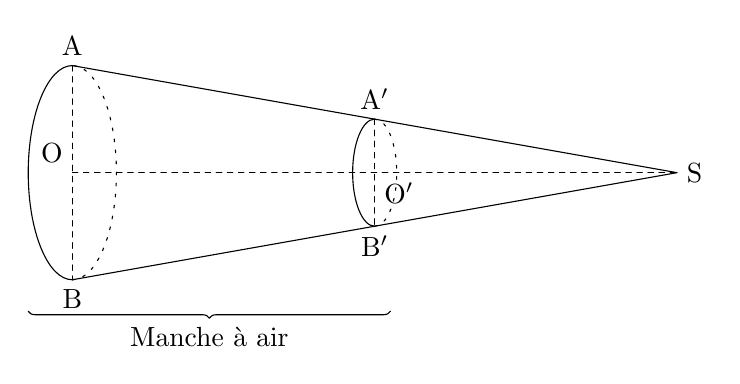
\begin{tikzpicture}[line cap=round,line join=round,x=0.8cm,y=0.8cm] %sur le sujet original x = 1cm, y = 1cm
\draw[] (0,1.7) arc (90:270:0.7 and 1.7);
\draw[dash pattern = on 1 pt off 3pt] (0,-1.7) arc (-90:90:0.7 and 1.7);
\draw[] (4.8,0.85) arc (90:270:0.35 and 0.85);
\draw[dash pattern = on 1 pt off 3pt] (4.8,-0.85) arc (-90:90:0.35 and 0.85);
\draw (0.,1.7)-- (9.6,0.) -- (0.,-1.7);
\draw [dash pattern = on 2 pt off 2pt] (0.,1.7)-- (0.,-1.7);
\draw [dash pattern = on 2 pt off 2pt] (4.8,0.85)-- (4.8,-0.85);
\draw [dash pattern = on 2 pt off 2pt] (0.,0.)-- (9.6,0.);
\draw[decorate,decoration={brace}] (5.05,-2.2)-- (-0.7,-2.2);
\draw (2.175,-2.3) node [ below]{Manche à air};
\draw [color=black] (0.,1.7) node [above]{A};
\draw [color=black] (0.,-1.7) node [below] {B};
\draw [color=black] (0.,0.) node [above left] {O};
\draw [color=black] (9.6,0.) node [right] {S};
\draw [color=black] (4.8,0.) node [below right] {O$'$};
\draw [color=black] (4.8,0.85) node [above] {A$'$};
\draw [color=black] (4.8,-0.85) node [below] {B$'$};

\end{tikzpicture}

On donne : AB = 60 cm, A$'$B$'$ = 30 cm, BB$'$ = 240 cm.

O est le centre du disque de la base du grand cône de sommet S.

O$'$ milieu de [OS], est le centre de la section de ce cône par un plan parallèle à la base.

B$'$ appartient à la génératrice [SB] et A$'$ appartient à la génératrice [SA].

\begin{enumerate}
	\item Démontrer que la longueur SB est égale à 480 cm.
	
	\item Calculer la longueur SO. On arrondira le résultat au centimètre.
	
	\item Calculer le volume d'air qui se trouve dans la manche à air.
	
On arrondira au centimètre cube.
\end{enumerate}

\emph{On rappelle les formules du volume d'un cône et l'aire d'un disque de rayon R :}

\hfill $V_{\mathrm{cône}} = \dfrac{1}{3} \times \text{aire de la base} \times \text{hauteur}$ \hfill et \hfill $A_{\mathrm{disque}} = \pi \times \text{R}^2$\hfill ~

\vspace{0,5cm}

